\section{Background and Related Work}
\label{sec:background}


    

% 介绍漏洞复现的定义、流程、难点
\subsection{Vulnerability Research}

\paragraph{Vulnerability Detection and Exploitation.}
%Automated vulnerability research is built on three intertwined lines. 
Vulnerability discovery progressed from random robustness testing and static buffer-overrun checking to concolic, whitebox, coverage-guided, and hybrid fuzzing~\cite{fuzz,wagner2000boon,godefroid2005dart,godefroid2008sage,bohme2016aflfast,stephens2016driller,qsym}. 
%Program analysis made these techniques applicable to complex binaries through symbolic execution, dynamic taint tracking, dynamic instrumentation, and reusable binary-analysis platforms~\cite{king1976symb,newsome2005taintcheck,nethercote2007valgrind,song2008bitblaze,s2e,angr}. 
Exploitation research 
%evolved from manual stack smashing and return-oriented programming 
aims to automatic exploit generation and autonomous cyber-reasoning systems~\cite{alephone1996stack,shacham2007rop,brumley2008patchaeg,avgerinos2011aeg,cha2012mayhem,mechanicalphish}. 
%These works establish how to find, analyze, and demonstrate the exploitability of a flaw once a program is available, whereas our setting additionally asks an agent to identify, acquire, build, and operationalize the affected target from only a CVE identifier.

\paragraph{IoT Vulnerability Detection.}
%For IoT devices, vulnerability reproduction is particularly challenging. 
Existing IoT vulnerability detection efforts predominantly rely on static analysis~\cite{karonte,satc,emtaint,hermescan,mango,nvwa}, which can identify candidate vulnerability paths but cannot confirm their triggerability in a real runtime environment~\cite{challenges}. Transforming static analysis reports into verified results requires dynamic validation on the actual firmware binary, a process that is largely manual and demands expert knowledge of firmware rehosting~\cite{firmadyne,firmae,greenhouse,pandawan}. The core difficulty lies in rehosting: proprietary firmware images are tightly coupled to specific hardware and often cannot be stably launched in emulation environments~\cite{fuzzware,firmafl}.

\paragraph{Vulnerability Reproduction.}
Vulnerability reproduction is the process of demonstrating that a known vulnerability exists by producing a proof-of-concept (PoC) that triggers the bug~\cite{cybergym}. Recent work has explored automating this process with LLM agents\cite{liu2026cve2poc,zhao2025systematic, krepro}. 
In practice, a security analyst reproduces a vulnerability starting from a CVE identifier by multi-steps and these steps are strictly sequential, so an early stage failure will block all downstream progress. This means that the full reproduction pipeline is far more demanding than the final triggering step alone.


\begin{figure}[t]
    \centering
    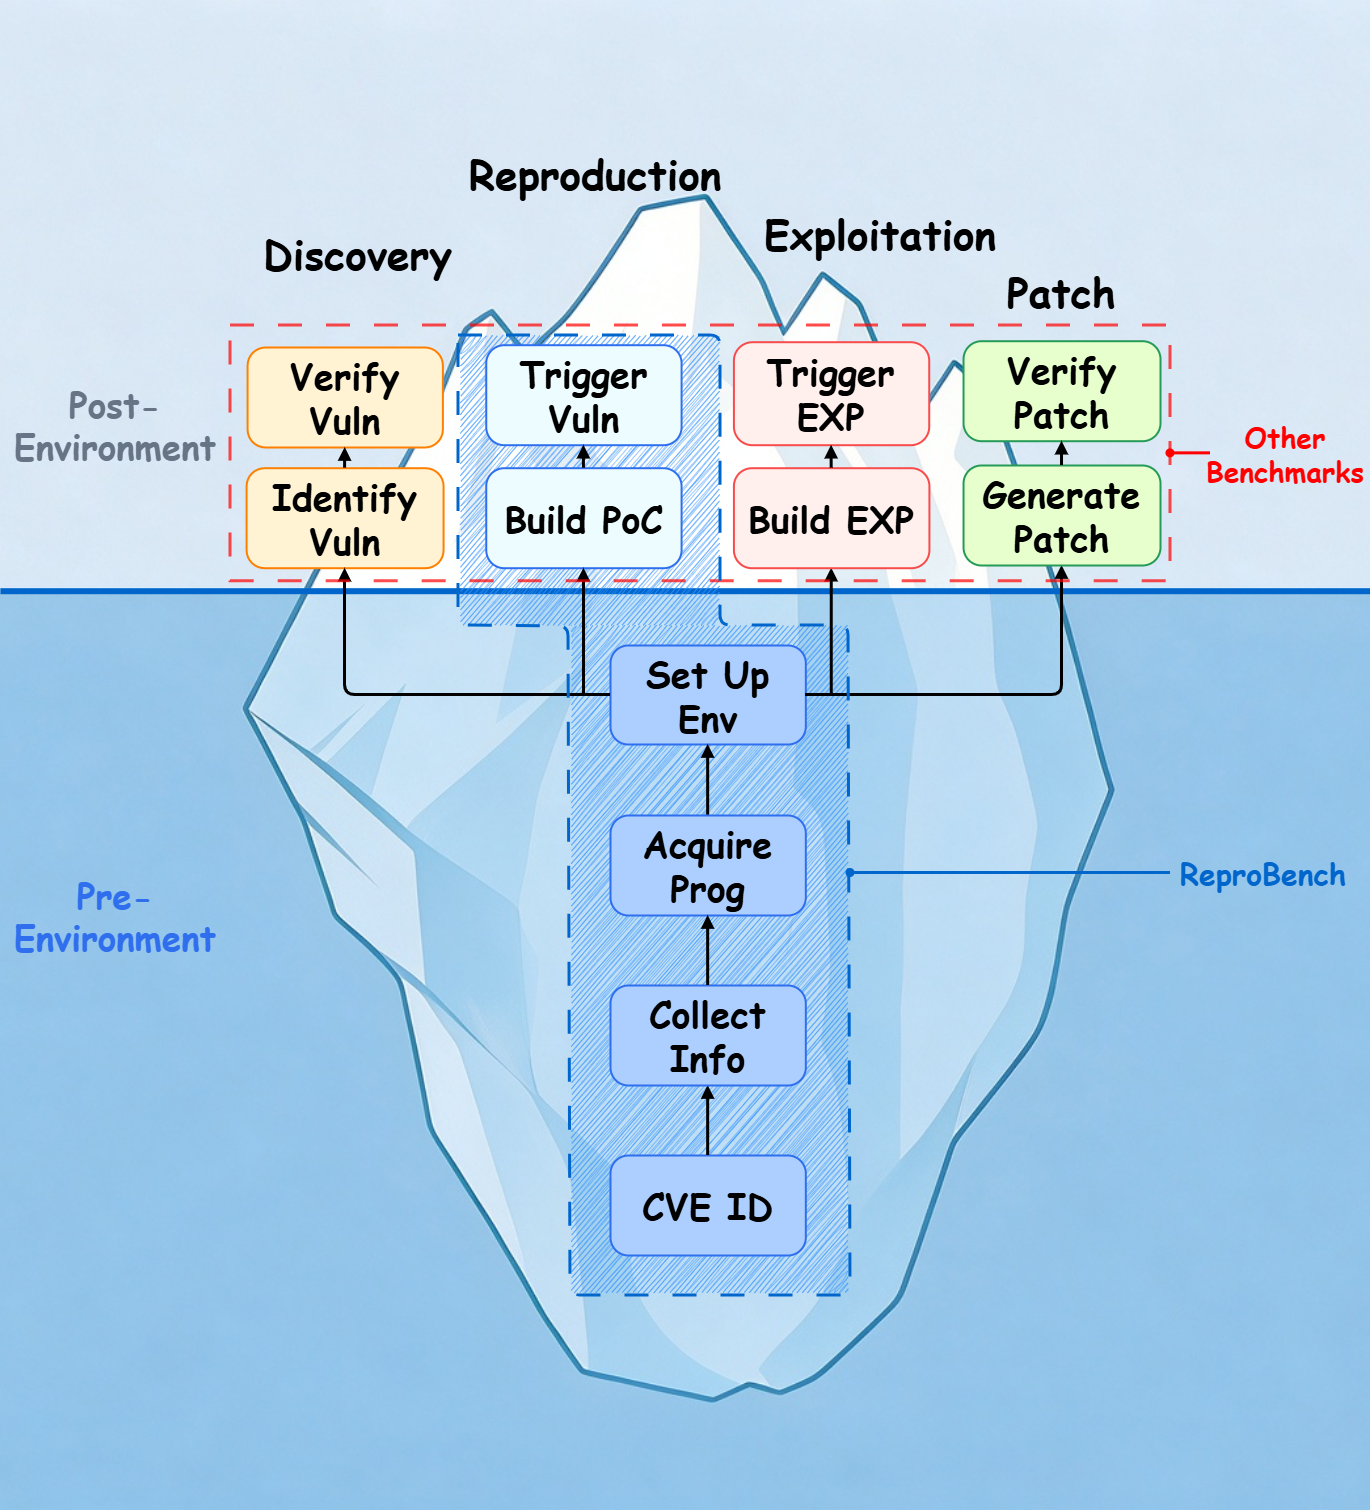
\includegraphics[width=\columnwidth]{figures/iceberg-v4.png}
    \caption{Comparison Between Existing Benchmarks and \sys{}.}
    \label{fig:iceberg}
    \end{figure}

% 网络安全benchmark，按四类漏洞任务分组
\subsection{Cybersecurity Benchmarks}
% Existing cybersecurity benchmarks can be grouped by which stage of the vulnerability lifecycle they evaluate: \emph{discovery} (finding an unknown vulnerability), \emph{reproduction} (producing a PoC that triggers a known vulnerability), \emph{exploitation} (escalating a bug into a concrete security impact), and \emph{patching} (generating a code fix). 
% For discovery, they usually provide the source code for
% the target programs (\cite{cybergym, cvebench, cybergyme2e, bountybench}). 
% For reproduction, beside the target program, they also need some more things, e.g., vulnerability description, a PoC script or a patch file (\cite{krepro, secbench}). 
% For exploitation and patching, they usually need a execution binary, a containerized or a running service before they conduct the evaluation (\cite{exploitbench, exploitgym, cybergyme2e}).
Existing cybersecurity benchmarks evaluate diverse security tasks---vulnerability discovery, reproduction, exploitation, and patching---but they differ most in what target access they assume at the start. 
Some hand the agent source code or a project repository~\cite{cybergym,secbench,cvebench,bountybench}; others provide patch context, vulnerability descriptions, or reference PoCs~\cite{krepro,secbench}; and still others start from a built binary, a container, or a running service~\cite{exploitbench,exploitgym,cybergyme2e}. 
In each case, the benchmark author has already prepared the affected target and corresponding environment, so the agent is scored only on the security task itself. 

\subsection{From-Scratch Reproduction Gap}
Based on above description, as illustrated in Figure~\ref{fig:iceberg}, all of these benchmarks operate in the post-environment setting: the target is already built, containerized, or running, and the agent is scored only on what it does after that starting line. Whether the agent can perform the full from-scratch reproduction pipeline---from a CVE identifier to triggering the vulnerability on the real target---remains an open question. \sys{} explores this question by making environment construction a scored phase of the reproduction pipeline and exposes the specific capabilities, common failure behaviors for the representative LLM agents.

\begin{figure*}[t]
    \centering
    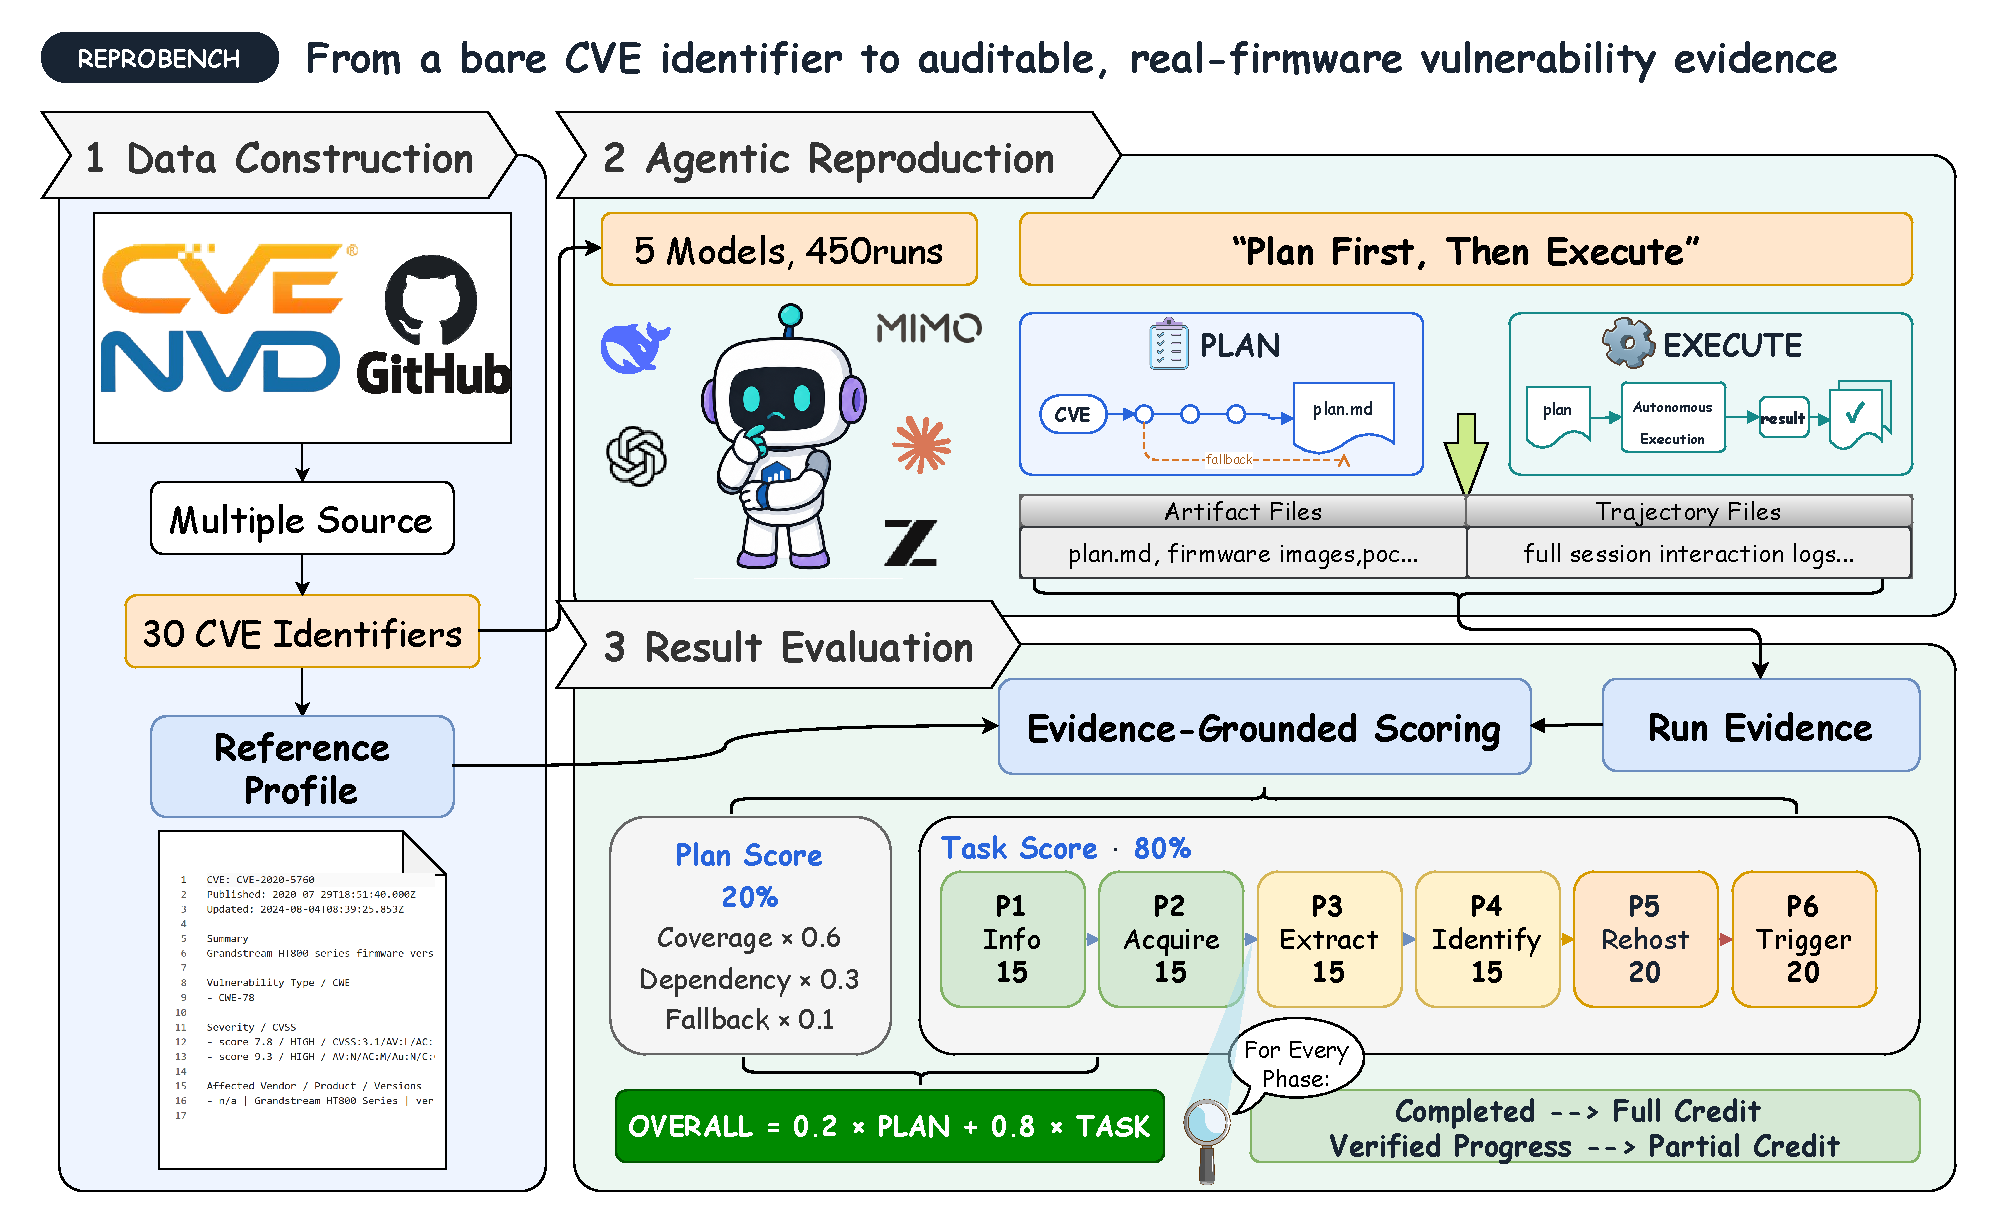
\includegraphics[width=0.8\textwidth]{figures/framework0724.pdf}
    \caption{Overview of the \sys{} pipeline. CVEs are curated and paired with public evidence. Agents receive only a CVE identifier and must plan, execute, and report. The scoring skill evaluates each run against the public evidence.}
    \label{fig:framework}
\end{figure*}